\chapter{Results of Experiments}

The various obfuscators defined earlier were iteratively applied to malware samples from the Contagio dataset. Based on the results obtained from VirusTotal, the obfuscators were selected for further application.

\section{Observations}

The VirusTotal website uploads a malware file to its database and then performs a scan using the various malware detectors associated with the website. 
Each uploaded file is hashed and stored in the database to reduce duplicate efforts and minimize scan times.

Due to this behavior, each time a file is loaded into the website to be scanned, the website will prompt if a similar file was scanned earlier. It was observed that as the number of obfuscators employed increased, the similarity between the obfuscated and un-obfuscated applications decreased.

If more than 2 certain obfuscators were applied, the VirusTotal website would not recognize the file as a previously recognized file. This observation was consistent throughout the different experiments conducted.

\section{Steps for Analyzing Malware Detectors}
The experiment was performed with certain operations being repeated in an iterative manner. The obfuscated malware files were prepared in advance. 
The steps are as follows:
\begin{itemize}
	\item Scan a malicious file using VirusTotal.
	\item Record the detection ratio.
	\item Apply obfuscator(s) on the selected malware file.
	\item Scan the obfuscated file using VirusTotal again.
	\item Record the new detection ratio.
\end{itemize}

Repeating the above steps helped us detect how robust and efficient malware detectors are. Ideally, the malware detector should not be affected by the obfuscators. The detection ratio should not be very different irrespective of whether the malware was obfsucated or not.

But the results indicated that almost all the malware files had a very high probability of being classified as a benign file, if they had sufficient obfuscation techniques applied to them.

\subsection{Metrics used}
We use the detection ratio provided by VirusTotal to determine the effectiveness of the Malware Obfuscators. As expected, the malware detectors are not resilient enough to detect variants of malware that have been slightly obfuscated.

\section{Obfuscators Application}

The results for applying each obfuscator were collected and only the significant results are shown here.

\subsection{Individual Obfuscators}

Application of individual obfuscators did not alter the detection ratio by a huge margin. A sample detection ratio for applying the "Renaming" obfuscator is shown in Fig. \ref{renaming}.

	 \vspace{3mm}
	 \begin{center}
	 	%\centering
	 	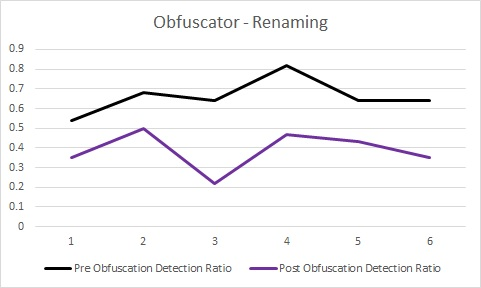
\includegraphics[width=0.8\textwidth]{renaming.jpg}
	 	\captionof{figure}{Single Obfuscator Usage - Renaming}
	 	\label{renaming}
	 \end{center}
	 \vspace{3mm}
	 
The results for the obfuscator "Reordering" are shown in \ref{reordering}.The detection ratio for this obfuscator is also lesser than for a normal malware. But with applying this obfuscator, the detection ratio is still reduced. 
	 
	 	 \begin{center}
	 	 	%\centering
	 	 	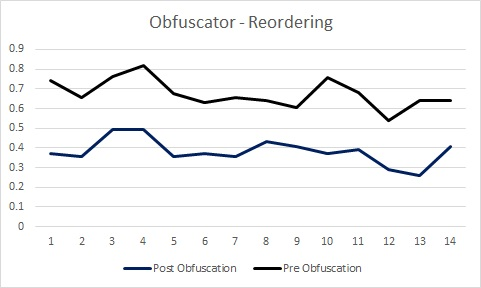
\includegraphics[width=0.8\textwidth]{reordering.jpg}
	 	 	\captionof{figure}{Single Obfuscator Usage - reordering}
	 	 	\label{reordering}
	 	 \end{center}
	 	 \vspace{3mm}
	 
\subsection{Multiple Obfuscators}

While individual obfuscators didn't provide much insight into the malware detection scores, it was observed that combining multiple obfsucators quickly decreased the detection ratio. 

In Fig. \ref{3Obfuscators}, the obfuscators Nop, Reordering, and Rename were applied to the files.

	 \vspace{3mm}
	 \begin{center}
	 	%\centering
	 	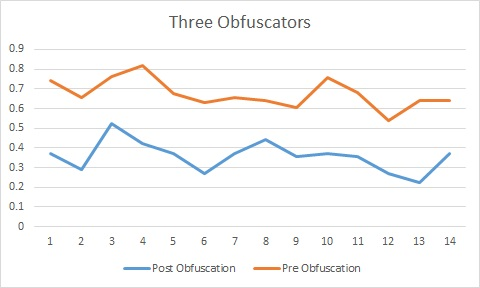
\includegraphics[width=0.8\textwidth]{3Obfuscators.jpg}
	 	\captionof{figure}{Detection Ratios with three obfuscators applied.}
	 	\label{3Obfuscators}
	 \end{center}
	 \vspace{3mm}

This certainly increased the obscurity of the malware files. The detection ratio for the obfuscated files in Fig.\ref{3Obfuscators} is much lesser than in Fig.\ref{renaming}. This could be attributed to the fact that a combination of weak obfuscators is still a strong enough challenge for malware detectors.

\subsection{All Obfsucators}	 

To make the results of the experiment certain, all the obfuscators in question were applied to a set of files. Keeping up with the consistency observed so far, the detection ratio dropped very low. This can be observed in Fig.\ref{detection}.
	 
 	 \vspace{3mm}
 	 \begin{center}
 	 	%\centering
 	 	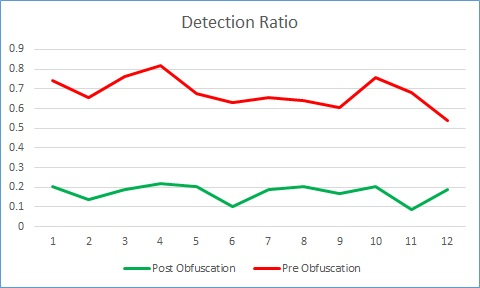
\includegraphics[width=0.8\textwidth]{detectionRatio.jpg}
 	 	\captionof{figure}{Pre and Post Obfuscation Results}
 	 	\label{detection}
 	 \end{center}
 	 \vspace{3mm}

This clearly shows that by increasing the number of obfuscators being applied to a malware, we can bring down the detection ratio of that particular file to a very low value. 	 